\chapter{The Project Panel}\label{lab:project}

The project panel helps the user to organize the recordings made within the different projects. On disk a project has the following fixed folder structure:

\begin{verbatim}
> root       // name of project
  |- data    // all data recorded within the project
    |- userA // recorded data of a single user
      |- 2010-12-06_14-46-12 // data of a single session
      |- 2010-12-06_14-51-34
    |- userB
    |- userX
  |- eval    // folders with evaluation results
    |- 2010-12-02_14-37-16
    |- 2010-12-02_14-42-45
  |- log     // log files
  |- opts    // option files
  |- stimuli // stimuli files
  |- train   // folders with trained models
    |- 2010-12-02_14-37-16
    |- 2010-12-02_14-42-45
\end{verbatim}

Since, the project panel automatically manages the folder and file structure of a project, it is usually not necessary to directly manipulate the file structure of a project.

\section{Overview}\label{lab:project_overview}

\begin{figure}[h]
\begin{center}
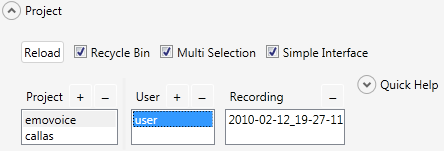
\includegraphics[scale=0.5]{pics/project_gui.png}
\end{center}
\vspace{-0.5cm}
\caption{The project panel.}
\label{fig:project_gui}
\end{figure}

The project panel is displayed on top and always visible (unless the user hides it by clicking the expander button on the top left). It is used to control the active project and browse recordings. Actions in the other panels often depend on the current selection.

The list on the most left shows a collection of all projects. A project holds recordings of one or more users and the trained models. Selecting a project from the list will load it. Users within the project are now displayed. The \texttt{+} button on the top of the list can be used to add new users. When a user name is selected according recordings are loaded. By holding down the ctrl-button and selecting several names it is possible to load recordings of multiple users (\texttt{Multi Selection} must be checked).

The \texttt{-} button above each list allows the user to delete selected items. In case of projects this will only cause the project to be excluded from the list of projects. For users and dates all related items (i.e. signal, annotation and sample files) will be deleted from disk. However, if the check box \texttt{Recycle Bin} is checked files will be moved to the recycle bin and can be recovered. The \texttt{Reload} button can be used to refresh the currently selected project.

\section{Creating a Project}\label{lab:project_create}

\begin{figure}[h]
\begin{center}
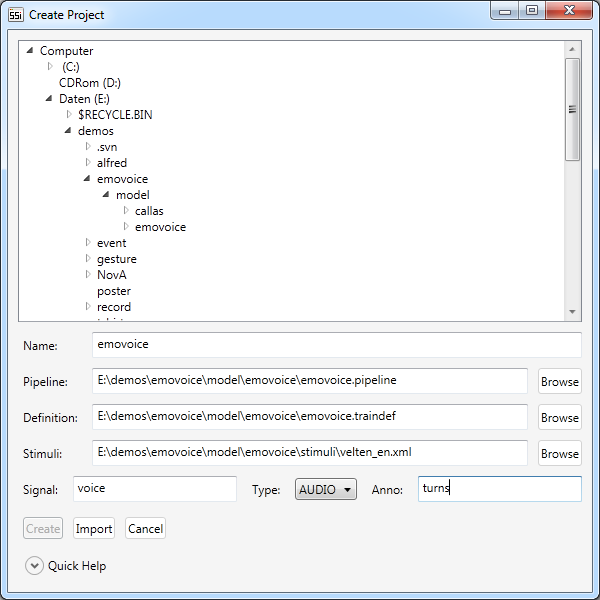
\includegraphics[scale=0.5]{pics/project_new.png}
\end{center}
\vspace{-0.5cm}
\caption{Dialogue for creating new or importing existing projects.}
\label{fig:project_new}
\end{figure}

The \texttt{+} button above the list of projects allows the user to either create a new project or import an existing project. A dialogue allows the user to enter the project settings.

First, the user must select a root folder on disk using the folder dialogue on top. Selecting a folder, which already contains a project will automatically activate the \texttt{'Import'} button. In this case now further settings are required. To create a new project enter a project name. A folder with this name will be automatically created. All recorded signals, annotations, samples and models, as well as, stimuli files will be created inside this folder. To move a project to another computer it is sufficient to copy the whole project folder and import it.

Next, a pipeline is set (ending to \texttt{*.pipeline}). Apart from the sensor and possible pre-processing steps, the pipeline must include a component \texttt{'ssi\_consumer\_MlpXml'}. It takes two signals as input: the signal we apply recognition to and an additional input (\texttt{xinput}), which is the trigger signal. The trigger signal indicates when a recognition event occurs. If the current sample value is non-zero recognition starts. When sample values become zero again recognition stops. E.g.\ in case of a speech recognizer the trigger signal would be the results of a voice activity detection (VAD). Though the component has several options, they will be automatically set except for the \texttt{type} option, which determines the storage format (0=ssi stream, 1=audio wav file, 2=video avi file). Here is an example for an audio signal triggered with a voice activity detection stored as an audio wav file:

\begin{lstlisting}[language=xml]
<consumer create="ssi_consumer_MlpXml" type="1">
   <input pin="audio" frame="0.2s" delta="0"/>
   <xinput size="1">
      <input pin="audio_vad"/>
   </xinput>
</consumer>
\end{lstlisting}

Now, a training definition file is selected (ending to \texttt{*.traindef}). It includes information on available feature extraction and classifier methods. Each \texttt{item} is given a unique name, which later on allows the user to choose between the different methods. Each item includes an optional \texttt{transform} and a mandatory \texttt{model} element. If a transformer is given it will be applied to the input stream before recognition in order to apply feature extraction. The following code carries on the above example and adds two classifiers, namely Naive Bayes and Support Vector Machines, together with a feature extraction component.

\begin{lstlisting}[language=xml]
<?xml version="1.0" ?>
<traindef ssi-v="1">
   <item name="ev-bayes">
      <transform create="ssi_feature_AudioFeatures"/>
      <model create="ssi_model_NaiveBayes"/>
   </item>	
   <item name="ev-svm">
      <transform create="ssi_feature_AudioFeatures"/>
      <model create="ssi_model_SVM"/>
   </item>	
</traindef>
\end{lstlisting}

In addition, the user has the option to select a stimuli file. A stimuli file stores slides displayed during a recording. They  usually include some instruction or stimuli and ask the user to perform certain actions or try to elicit certain behaviour. Each slide consists of a source, a trigger and a label. The source defines the content of the slide, which will be displayed as a html file in the web browser. The trigger defines how or when the transition to the next slide will happen. And the label is a description of the action or desired user state. Stimuli files follow a certain xml structure (see Table \ref{tab:stimuli_source} and \ref{tab:stimuli_trigger} for available definitions):

\begin{lstlisting}[language=xml]
<stimuli>
  <list size="x"> // number of slides in the stimuli
    <slide label="xxxxx"> // a single slide
        <source id="x" .../> // what is displayed
        <trigger id="x" .../> // how long is it displayed
    </slide>
    ...
  </list>
</stimuli>
\end{lstlisting}

\begin{table}
\begin{tabular}{clp{11cm}}
{\bf id} & {\bf description} & {\bf example} \\
\hline
\texttt{Text} & plain text & \texttt{<source id="Text" text="do this and that.." color="00FF00" size="5"/> } \\
\texttt{Code} & html code & \texttt{<source id="Code" code="\&lt;h1\&gt;do something else..\&lt;/h1\&gt;" /> } \\
\texttt{URL} & linked page & \texttt{<source id="URL" url="http://hcm-lab.de" /> } \\
\hline
\end{tabular}
\caption{Supported definitions for stimuli sources.}
\label{tab:stimuli_source}
\end{table}

\begin{table}
\begin{tabular}{clp{7.6cm}}
{\bf id} & {\bf description} & {\bf example} \\
\hline
\texttt{Button} & waits for user to press button & \texttt{<trigger id="Button" /> } \\
\texttt{Timer} & waits x seconds & \texttt{<trigger id="Timer" seconds="3"/> } \\
\texttt{Event} & waits for x user events & \texttt{<trigger id="Event" number="3"/> } \\
\hline
\end{tabular}
\caption{Supported definitions for stimuli trigger.}
\label{tab:stimuli_trigger}
\end{table}

Finally, the type of the signal has to be selected. It has to correspond to the one used in the pipeline, i.e.\ stream, audio or video. Name of signal and annotation can be chosen arbitrarily.

When the user presses \texttt{Create} all files will be copied to the root folder and the project settings are stored in a file \texttt{'modelui.project.xml'} located in the root folder of the project. Afterwards the new project is added to the list of projects and loaded.

